% \documentclass[letterpaper,12pt]{report}
% \usepackage[pdftex]{graphicx}
% \usepackage[spanish]{babel}
% \usepackage[latin1]{inputenc}
% \pagestyle{plain}
% 
% \begin{document}
% \addtolength{\textwidth}{-3cm}
% \begin{figure}
% \chapter{UML}

%%%%%%%%%%%%%%%%%%%%%%%%%% CLASE  C45 %%%%%%%%%%%%%%%%%%%%%%%%%%%%%%%%%%%%%%%%%%%%
\begin{figure}
\subsubsection{Clase C45}
%\addtolength{\textwidth}{-3cm}
%\centering
%\includegraphics[width=1.2\textwidth]{imgsSecuencia/c45/C45Clear.png}
%\caption{C45Clearequalsparcializados}
%\end{figure}
%\newpage
%\begin{figure}
\centering
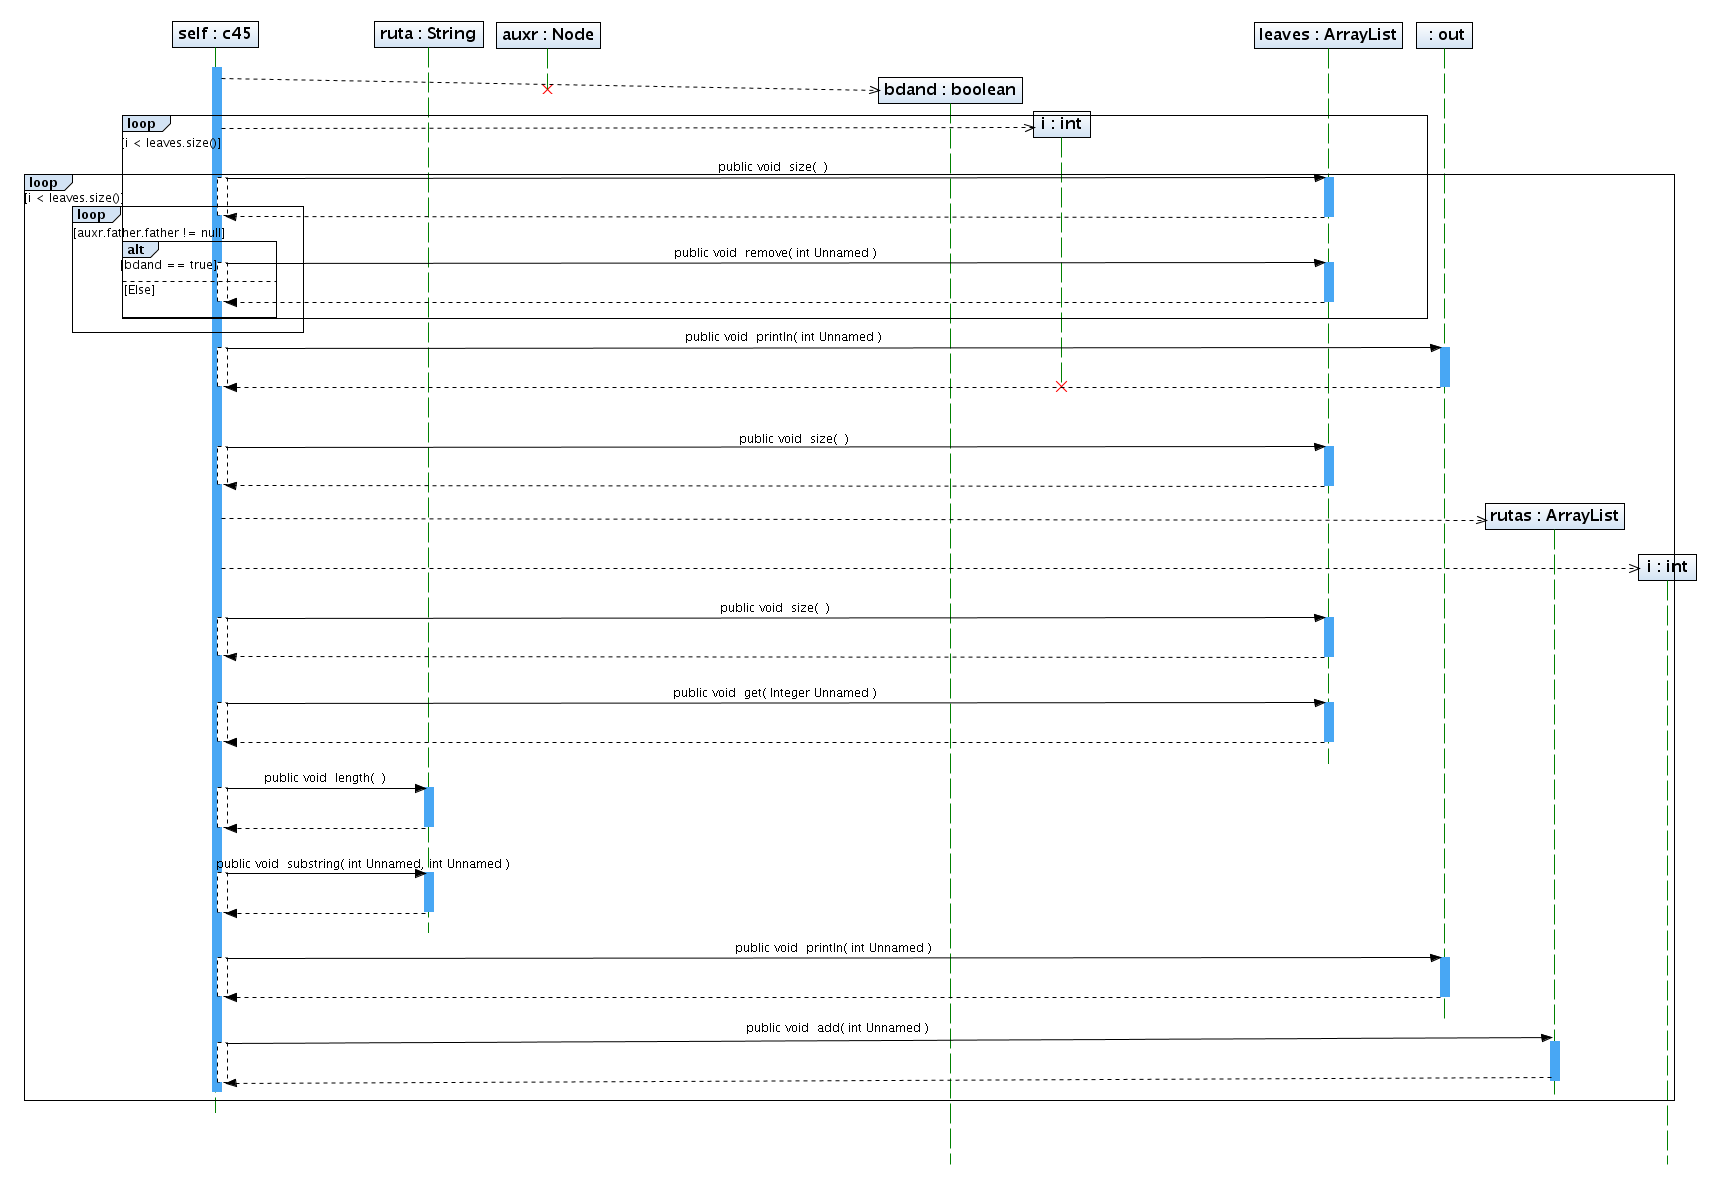
\includegraphics[angle=90, width=0.7\textwidth]{imgsSecuencia/c45/C45Rules.png}
\caption{C45Rules}
\end{figure}
\newpage


%%%%%%%%%%%%%%%%%%%%%%%%%% CLASE  myHasMap %%%%%%%%%%%%%%%%%%%%%%%%%%%%%%%%%%%%%%%%%%%%
\begin{figure}
\subsubsection{Clase myHasMap}
\centering
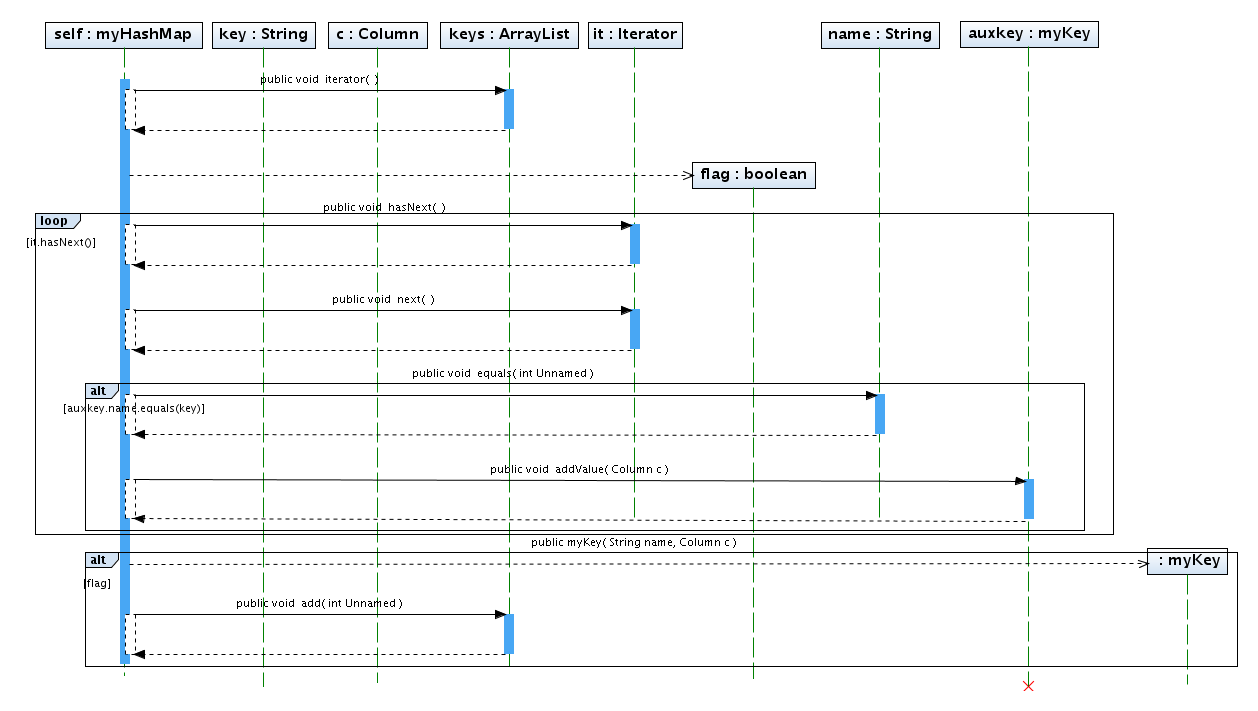
\includegraphics[angle=90, width=0.6\textwidth]{imgsSecuencia/myHasMap/addColumn.png}
\caption{addColumn}
\end{figure}
\newpage
\begin{figure}
\centering
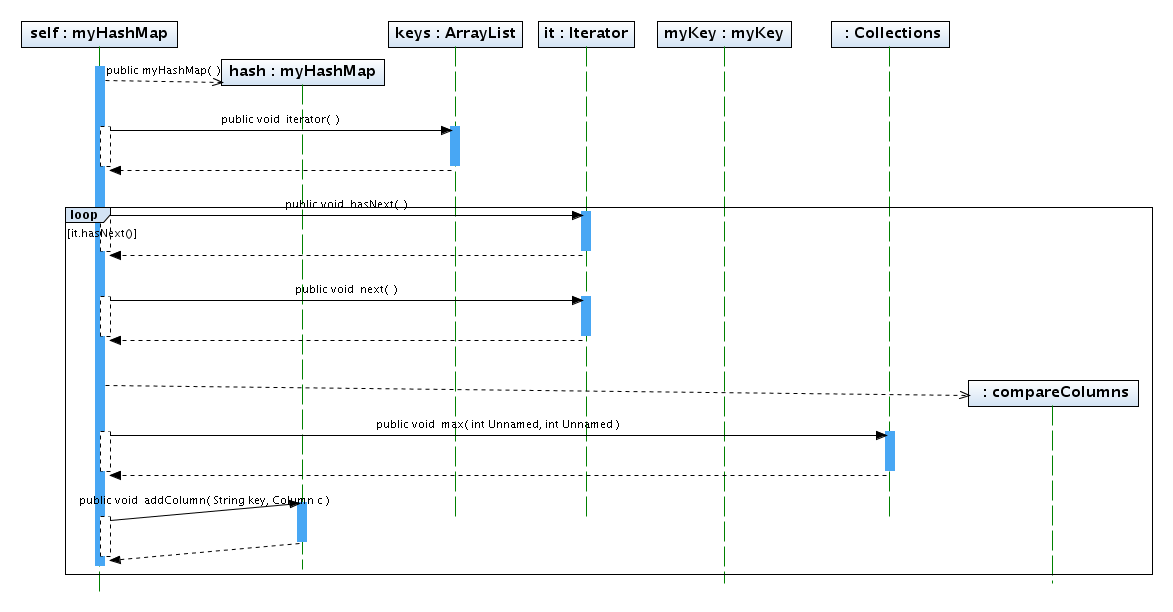
\includegraphics[angle=90, width=0.6\textwidth]{imgsSecuencia/myHasMap/SearchColumn.png}
\caption{SearchColumn}
\end{figure}
\newpage


%%%%%%%%%%%%%%%%%%%%%%%%%% CLASE  Route %%%%%%%%%%%%%%%%%%%%%%%%%%%%%%%%%%%%%%%%%%%%

\begin{figure}
\subsubsection{Clase Route}
\centering
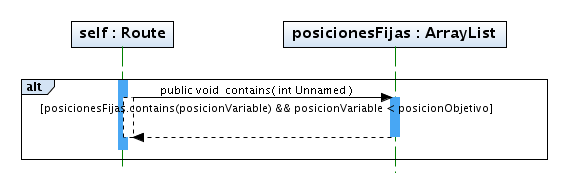
\includegraphics[width=1\textwidth]{imgsSecuencia/Route/avanceVariable.png}
\caption{avanceVariable}
\end{figure}
\newpage
\begin{figure}
\centering
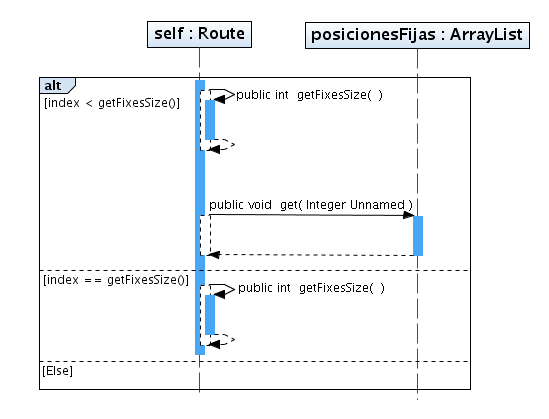
\includegraphics[width=1\textwidth]{imgsSecuencia/Route/getIndex.png}
\caption{getIndex}
\end{figure}
\newpage
\begin{figure}
\centering
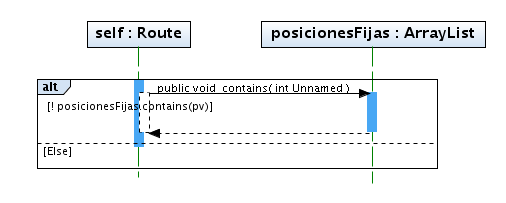
\includegraphics[width=1\textwidth]{imgsSecuencia/Route/setPoscicionVariable.png}
\caption{setPoscicionVariable}
\end{figure}
\newpage

%%%%%%%%%%%%%%%%%%%%%%%%%% CLASE  TreeCounter %%%%%%%%%%%%%%%%%%%%%%%%%%%%%%%%%%%%%%%%%%%%
\begin{figure}
\subsubsection{Clase TreeCounter}
\centering
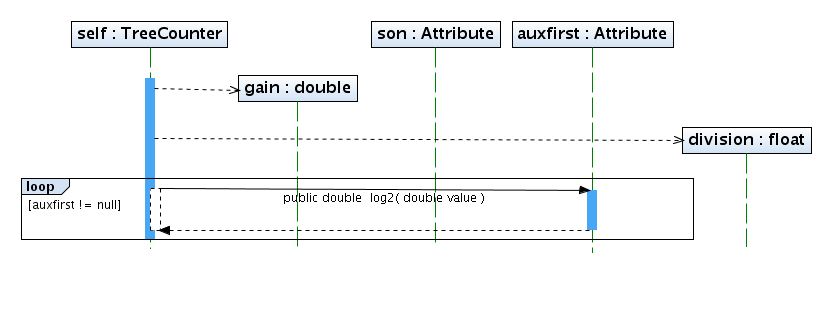
\includegraphics[width=1\textwidth]{imgsSecuencia/TreeCounter/gananciaInicial.png}
\caption{firstGain}
\end{figure}
\newpage
\begin{figure}
\centering
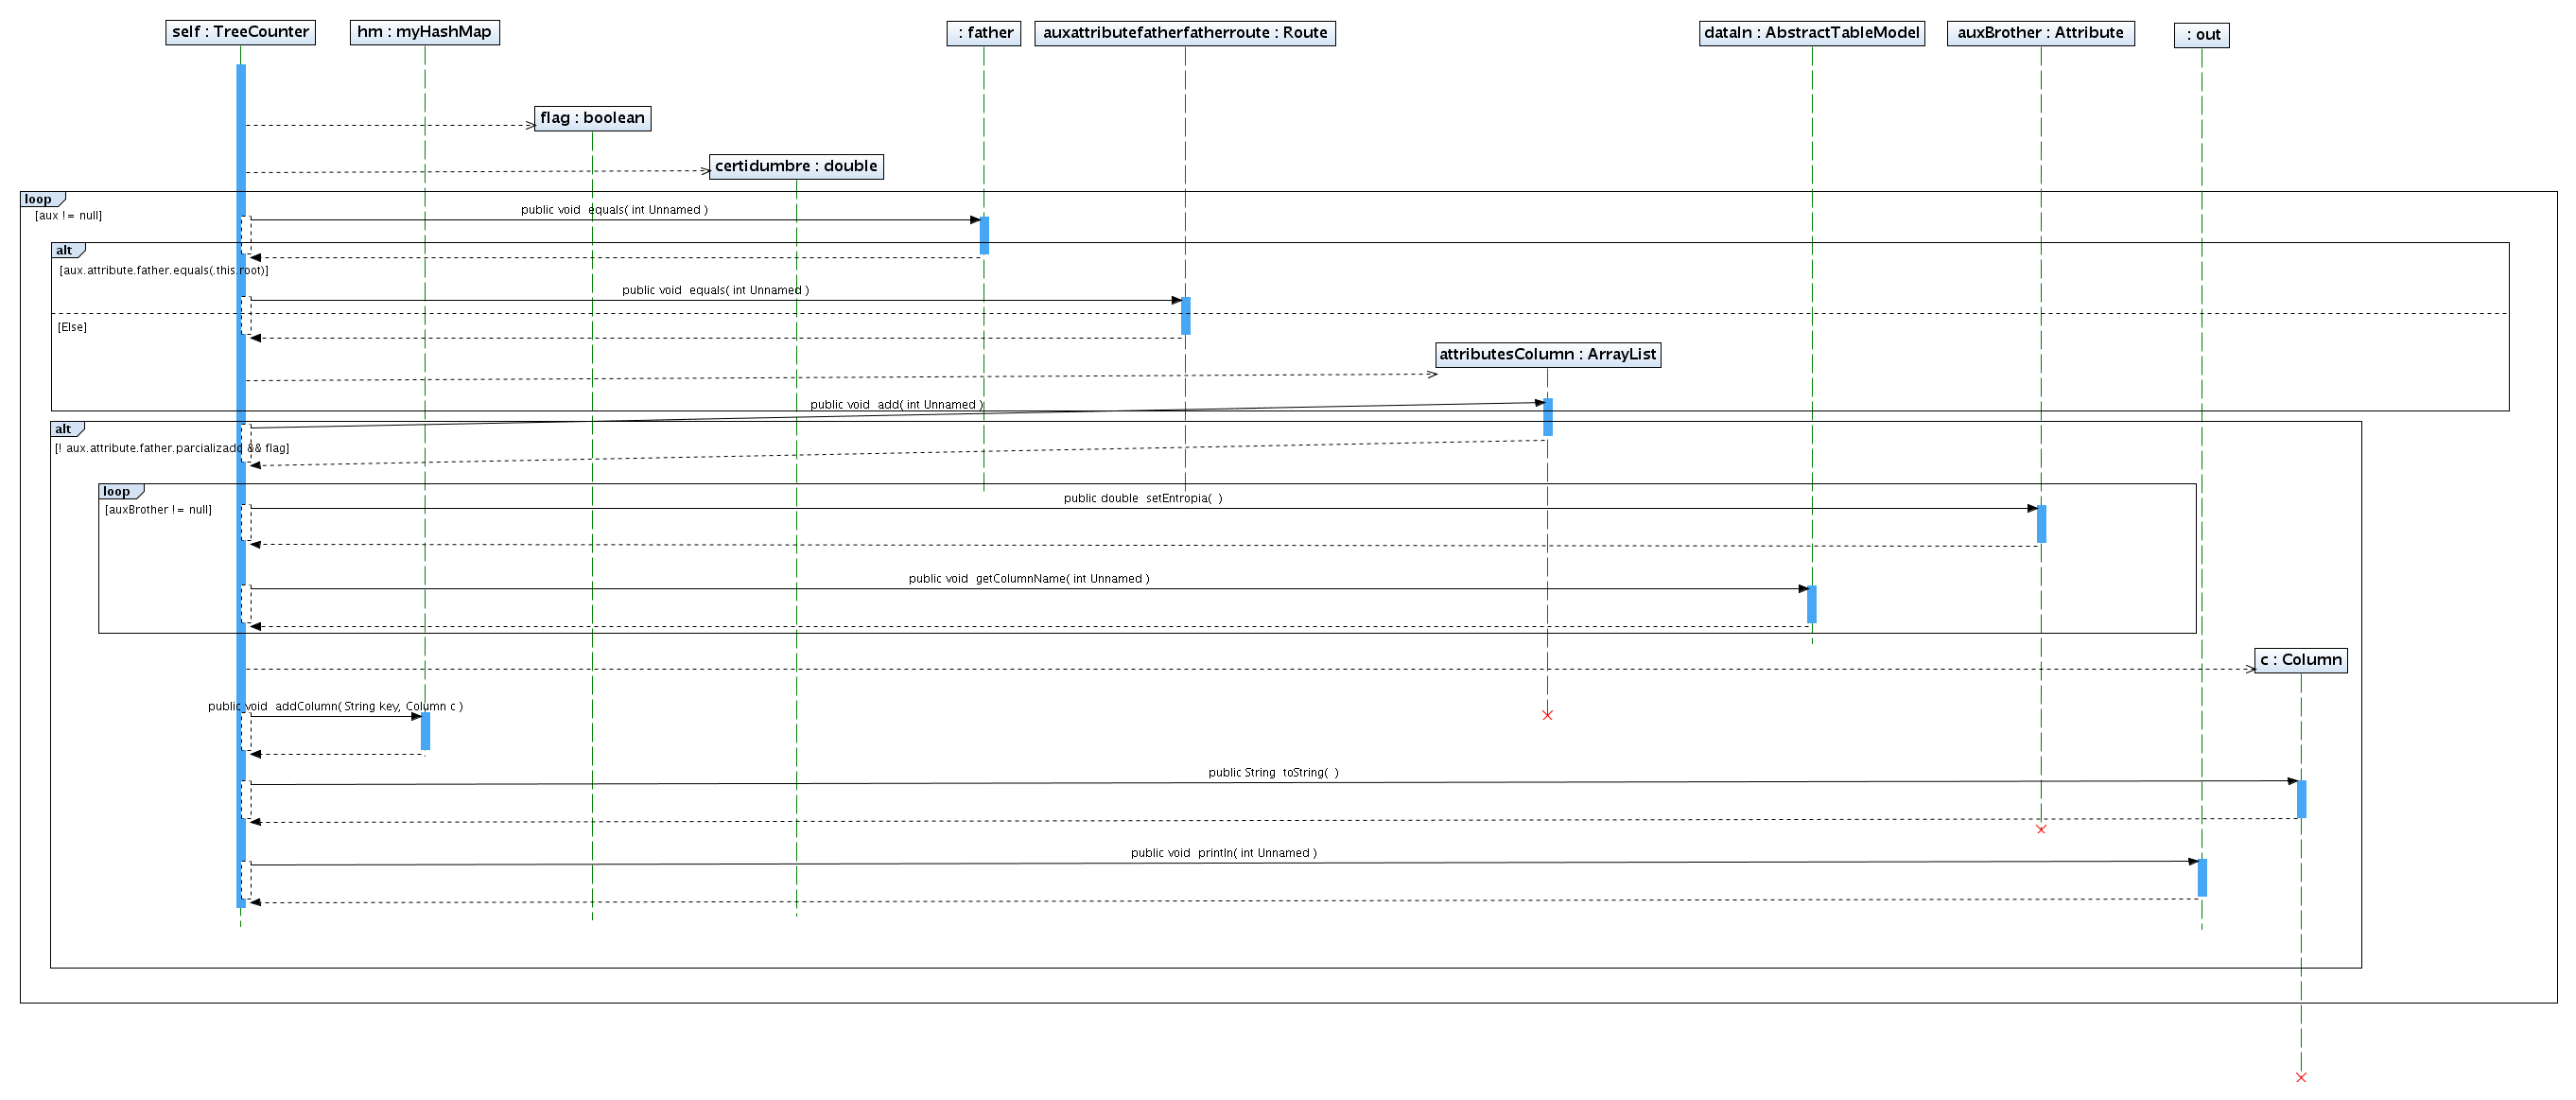
\includegraphics[angle=90, width=0.5\textwidth]{imgsSecuencia/TreeCounter/ganancia.png}
\caption{gain}
\end{figure}
\newpage
%\begin{figure}
%\centering
%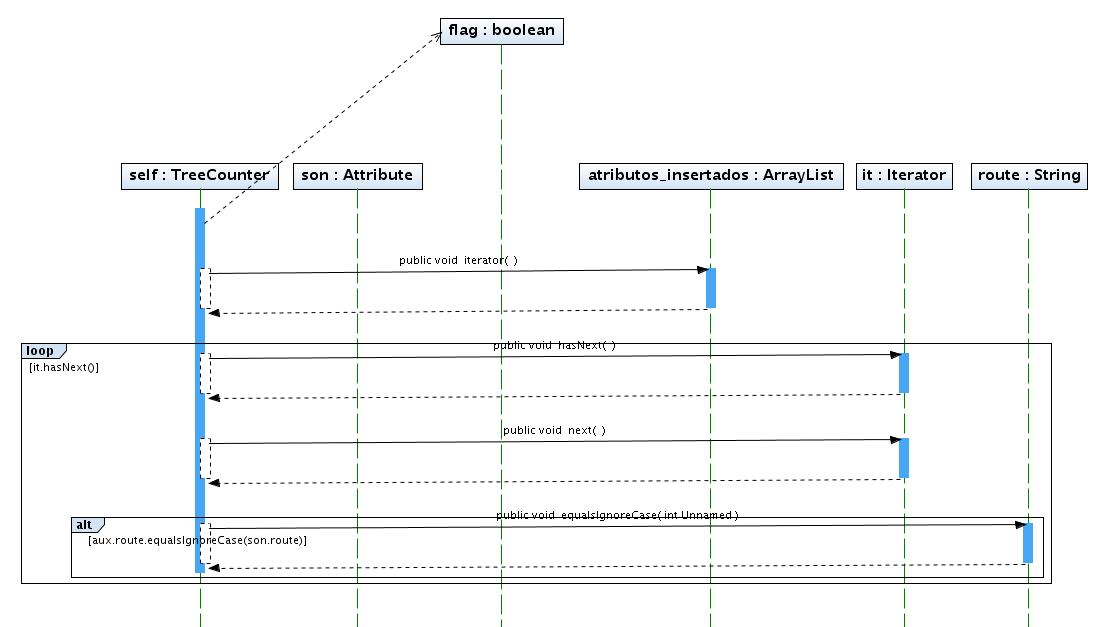
\includegraphics[width=1\textwidth]{imgsSecuencia/TreeCounter/searchAttribute.png}
%\caption{searchAttribute}
%\end{figure}
%\newpage
%\begin{figure}
%\centering
%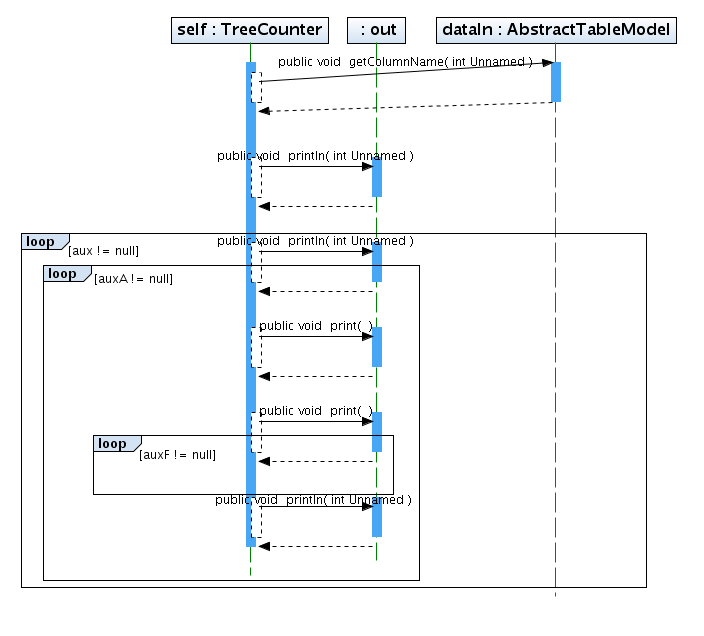
\includegraphics[width=1\textwidth]{imgsSecuencia/TreeCounter/seeTree.png}
%\caption{seeTree}
%\end{figure}
%\newpage

%%%%%%%%%%%%%%%%%%%%%%%%%% CLASE  Attribute %%%%%%%%%%%%%%%%%%%%%%%%%%%%%%%%%%%%%%%%%%%%

\begin{figure}
\subsubsection{Clase Attribute}
\centering
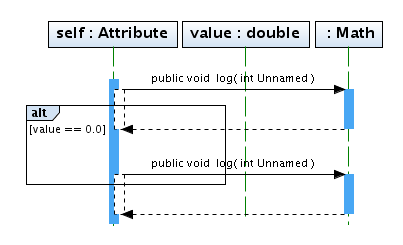
\includegraphics[width=1\textwidth]{imgsSecuencia/Attribute/log2.png}
\caption{log2}
\end{figure}
\newpage
\begin{figure}
\centering
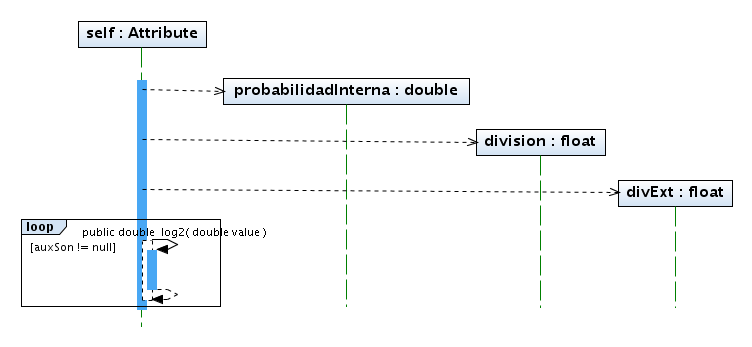
\includegraphics[width=1.2\textwidth]{imgsSecuencia/Attribute/setEntropia.png}
\caption{setEntropia}
\end{figure}
\newpage


%%%%%%%%%%%%%%%%%%%%%%%%%% CLASE  Node %%%%%%%%%%%%%%%%%%%%%%%%%%%%%%%%%%%%%%%%%%%%

\begin{figure}
\subsubsection{Clase Node}
\centering
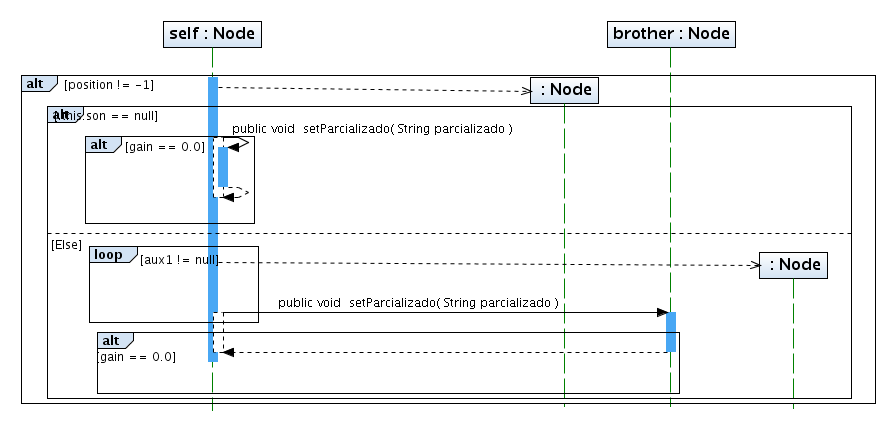
\includegraphics[width=1.2\textwidth]{imgsSecuencia/Node/addSon.png}
\caption{addSon}
\end{figure}
\newpage
\begin{figure}
\centering
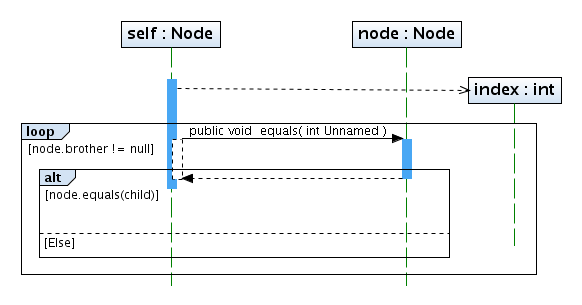
\includegraphics[width=1\textwidth]{imgsSecuencia/Node/getIndexOfChild.png}
\caption{getIndexOfChild}
\end{figure}
\newpage
% 
% \end{document}
